Several tasks exist around the modelling of human motion and the given task usually dictates the shape of the model to a certain extent.

One such example is animating a human 3D mesh to conform with input from a game controller or equivalent keyboard input. This task is of particular interest for the video game industry. One such model is a phase-functioned neural network, wherein multiple networks are samples in a phase, as to mimic the repetitive nature of walking~\cite{holden2017}. This approach can be extended to other tasks, such as playing basketball~\cite{starke2020}. This approach values being able to run in real-time higher than animation quality. This makes it ideal for video games, but less ideal for other applications where the animations are typically produced in advance and as such there is no requirement for real-time production.

Another example is motion prediction, where the model is given a sequence of human poses and asked to generate future human poses. This is of particular interest for the autonomous car industry, but also has a potential impact for all industries that produce animations, which includes industries working with: movies, video games, entertainment, infotainment, education, etc. As auto-completing an animation could potentially speed up the time it takes to produce a finished animation. A common approach to this task is to use recurrent neural networks~\cite{hu2020predicting, jain2016structuralrnn}. Generative adversarial networks (GAN) are commonly used in image based generative tasks, such as generating human faces \cite{karras2019stylebased}. GANs have been shown to also be effective for human motion prediction~\cite{ruiz2019human}.

In-painting of human motion or interpolation between two different human motions can be considered a special case of motion prediction, where the model gets both the past and future motion, instead of only getting past motion. This could be used to help speed up the animation of humanoids for video games, movies, etc. It seems that data on this particular task is relatively sparse.

GANs have seen great success in image in-painting~\cite{bau2019ganpaint} and image generation~\cite{karras2019stylebased}. The core idea of GANs being that you train two models in tandem. One model learns to generate content and the other learns to distinguish between generated content and the ground truth. This allows for a sort of ping-pong training that has yielded great results for image models and human motion models.

Recently variational autoencoders~\cite{kingma2014autoencoding} (VAE) have been shown to produce results that are as good as the state of the art results produced by GAN models~\cite{razavi2019generating}. The VAE is built upon the concept of an autoencoder. An autoencoder is a model that encodes a given input to a latent space and then decodes the latent vector back into something that resembles the input. The latent space of an autoencoder model is analogous to the input given to the generator of a GAN model. Giving random values to the decoder of an autoencoder or as input to the generator of a GAN can be used to generate random realistic outputs. Editing data using GANs and traditional autoencoders is limited. Some models allow for blending between existing data and some support a limited kind of arithmetic~\cite{karras2019stylebased}. For example: Subtracting a picture of someone with glasses with a picture of someone without glasses, and then adding that to a picture of someone to add glasses on him. Traditional autoencoders have no builtin way of ensuring that the latent space is continuous. This means that random sampling or interpolation between two latent values might yield a latent value that would never have been created by the encoder, see \autoref{fig:cmp} for a visualization. Such a latent value is unlikely to yield good results. Such a latent space is said to lack regularity. VAEs are autoencoders that are specifically built to add regularity to the latent space. This means that the latent space of a VAE is continuous and can thus be randomly sampled to generate random values, and the interpolation between two latent values is going to always produce valid intermediate latent values. It is plausible that training a VAE for a given domain of human motion, for example walking, could be used for animation inpainting of that given motion. This is accomplished by encoded the human pose at the beginning and end of the gap to be filled. Blending between the two latent values then gives an approximation of what the human motion might look like in the gap. This is restrained by VAE not having any temporal component and by only using a single data point for the beginning and end of the gap. As such it is unlikely to work well for long gaps in motion.


\begin{figure}[h]
\centering
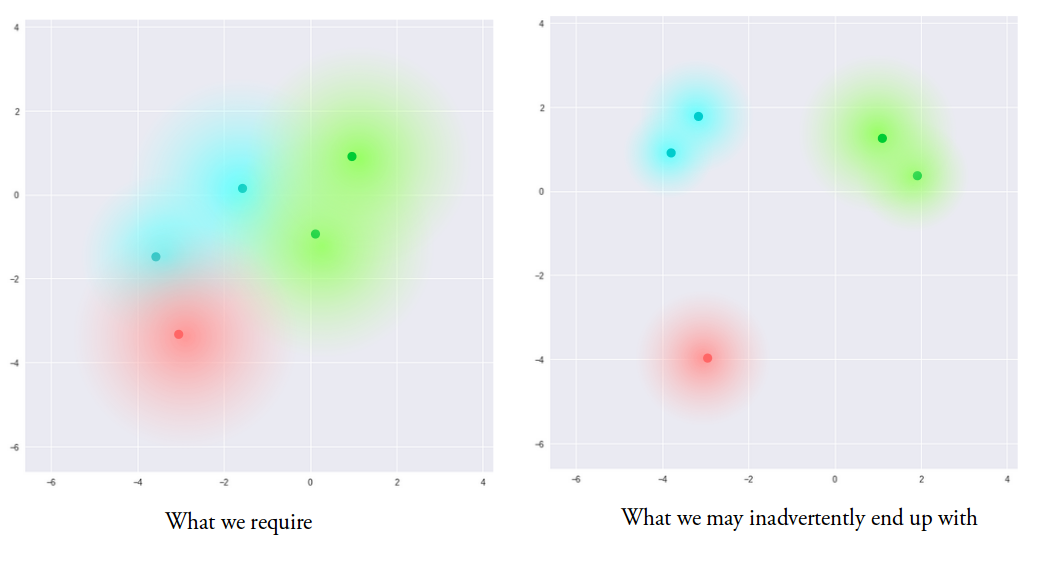
\includegraphics[width=0.5\textwidth]{img/cmp}
\caption{Visualization of a regular (left) and a non-regular (right) latent space. This figure is from \cite{shafkat2018}.}
\label{fig:cmp}
\end{figure}
